% Created 2023-03-04 Sat 11:07
% Intended LaTeX compiler: pdflatex
\documentclass[11pt]{article}
\usepackage[utf8]{inputenc}
\usepackage[T1]{fontenc}
\usepackage{graphicx}
\usepackage{longtable}
\usepackage{wrapfig}
\usepackage{rotating}
\usepackage[normalem]{ulem}
\usepackage{amsmath}
\usepackage{amssymb}
\usepackage{capt-of}
\usepackage{hyperref}
\author{Yusheng Zhao}
\date{\today}
\title{Homework 1}
\hypersetup{
 pdfauthor={Yusheng Zhao},
 pdftitle={Homework 1},
 pdfkeywords={},
 pdfsubject={},
 pdfcreator={Emacs 28.2 (Org mode 9.6)}, 
 pdflang={English}}
\begin{document}

\maketitle
\tableofcontents


\section{Problem 1}
\label{sec:org268bc4b}
\begin{itemize}
\item Name: SPERM WHALE MYOGLOBIN F46V N-BUTYL ISOCYANIDE AT PH 9.0
\item ID: 101M
\begin{figure}[htbp]
\centering
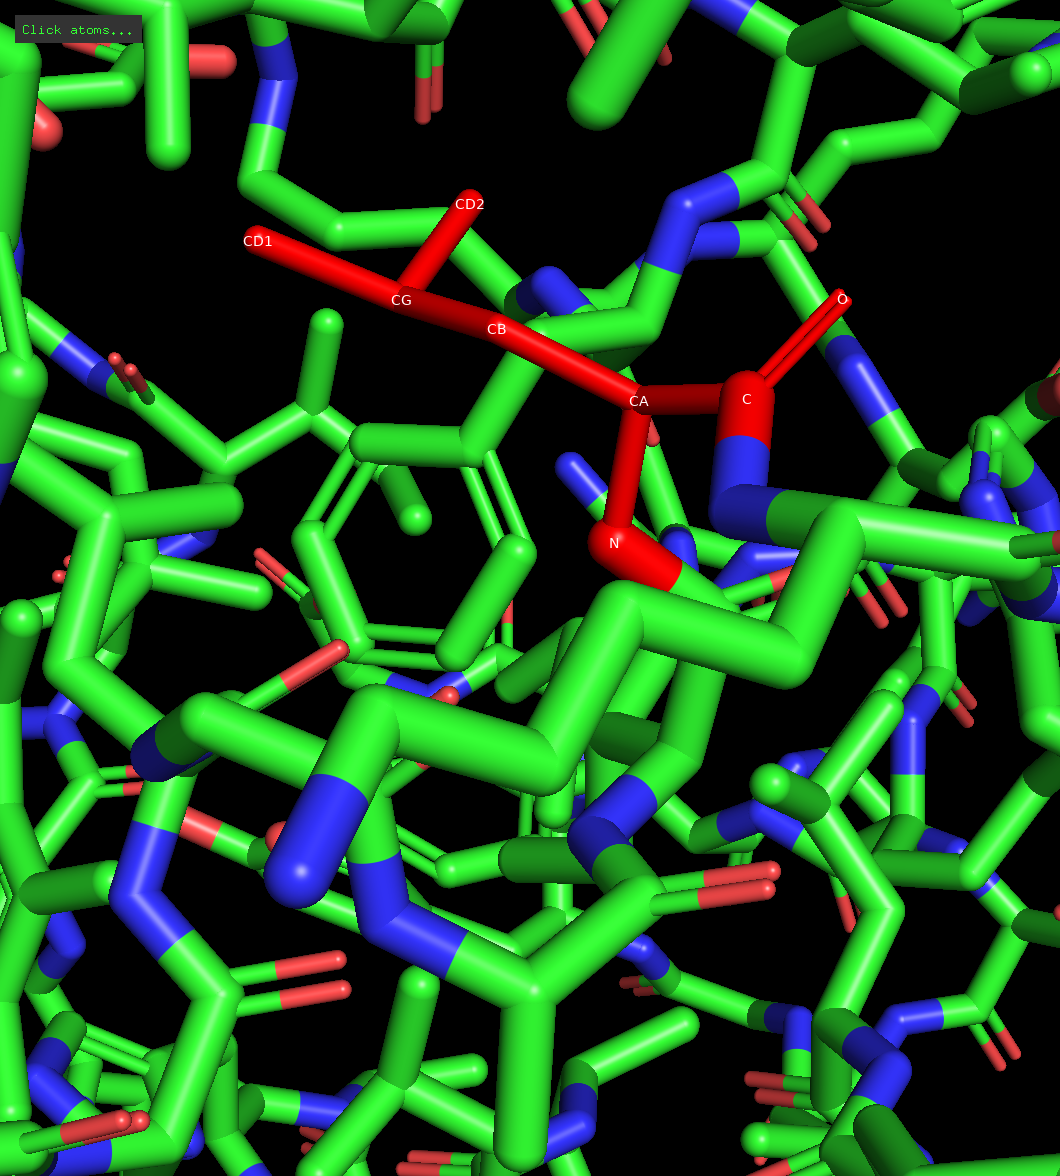
\includegraphics[width=.9\linewidth]{./sticks.png}
\caption{Illustration of molecule with sticks, atoms names of one amino acid labeled.}
\end{figure}

\begin{figure}[htbp]
\centering
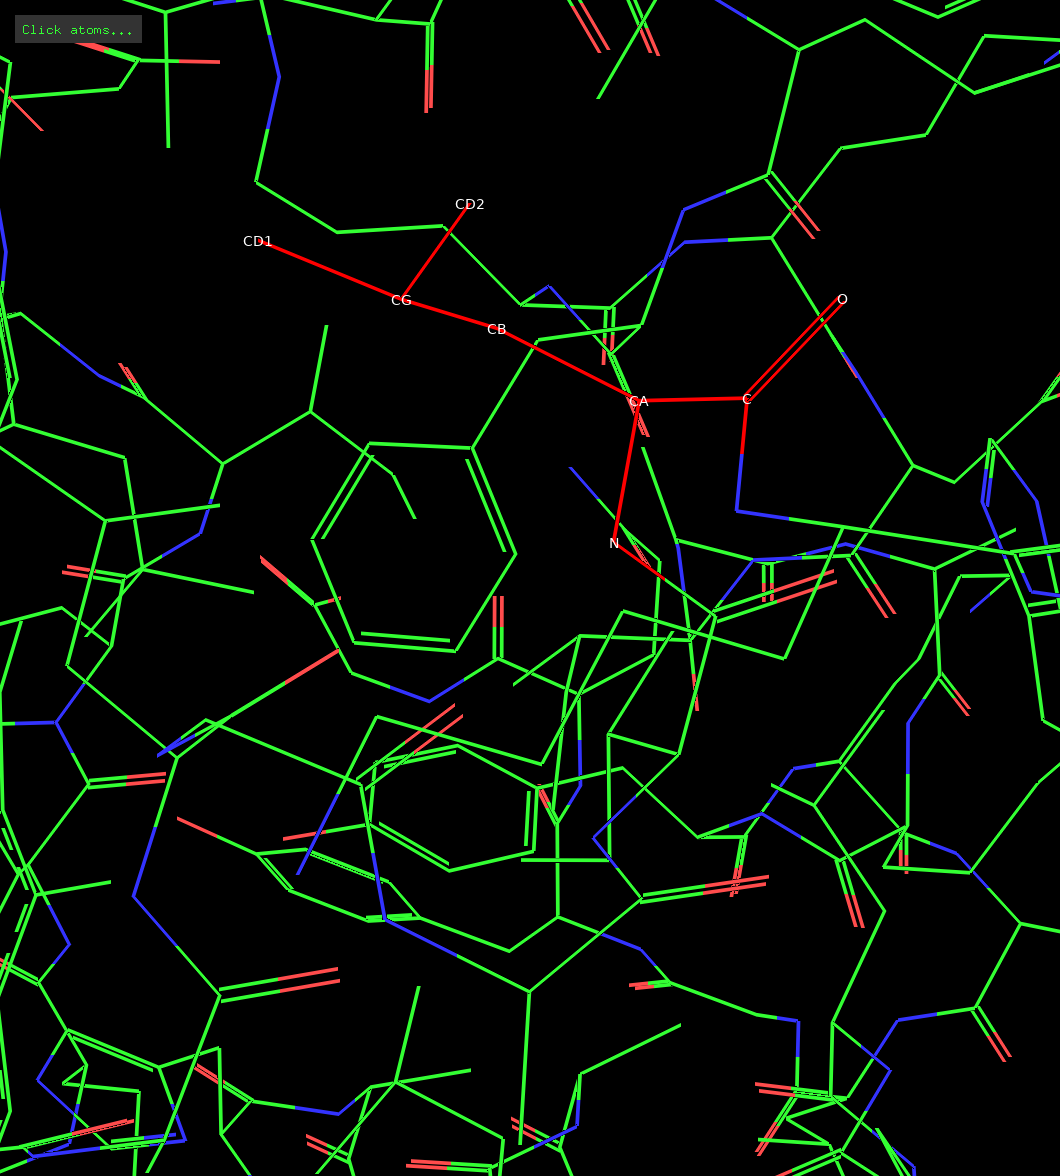
\includegraphics[width=.9\linewidth]{./lines.png}
\caption{Illustration of molecule with lines, atoms of one amino acid labelled}
\end{figure}

\begin{figure}[htbp]
\centering
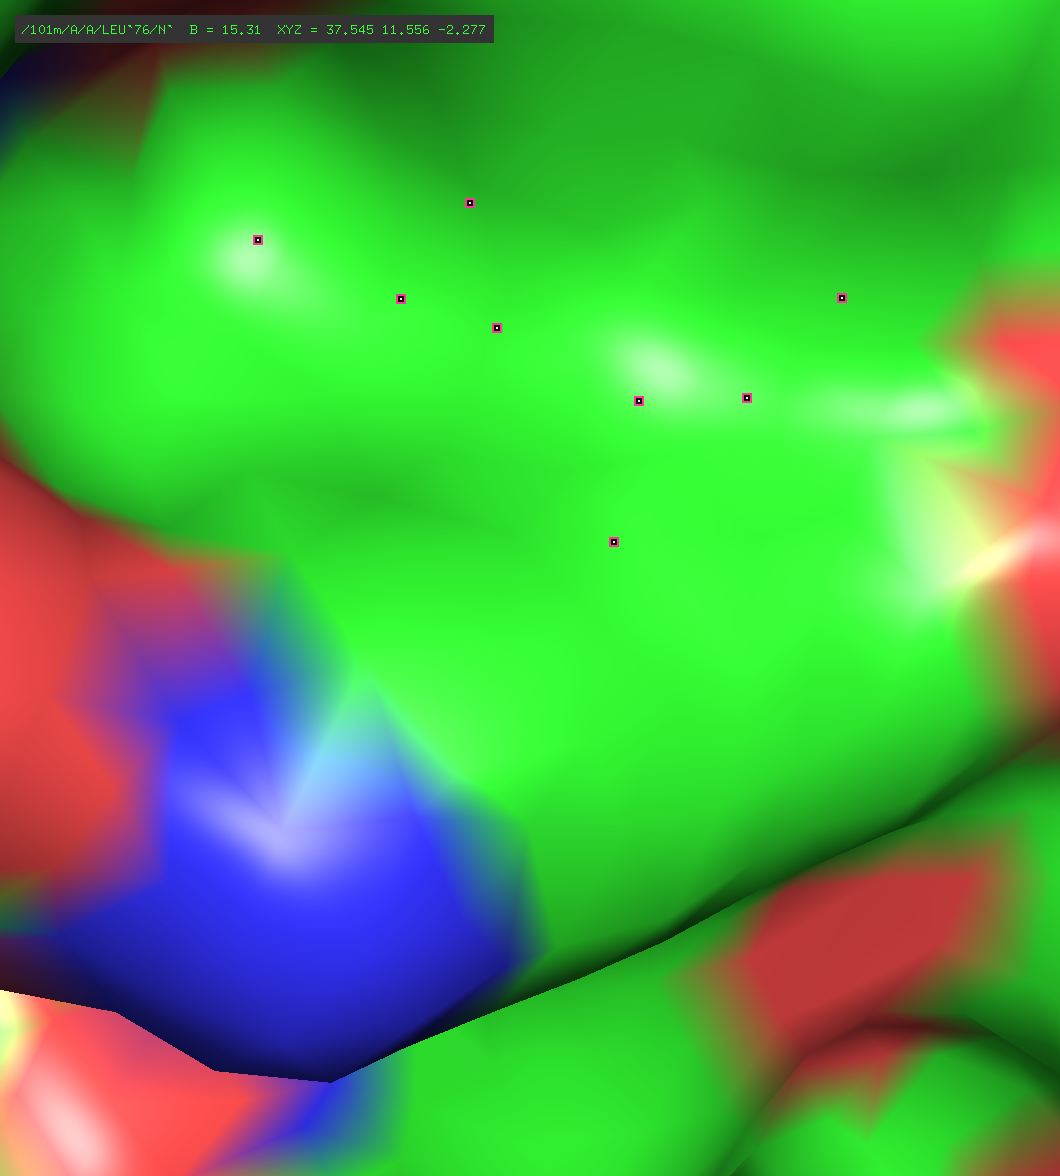
\includegraphics[width=.9\linewidth]{./surfaces.png}
\caption{Illustration of molecule with surfaces, atoms and names hidden under surface}
\end{figure}
\end{itemize}

\begin{figure}[htbp]
\centering
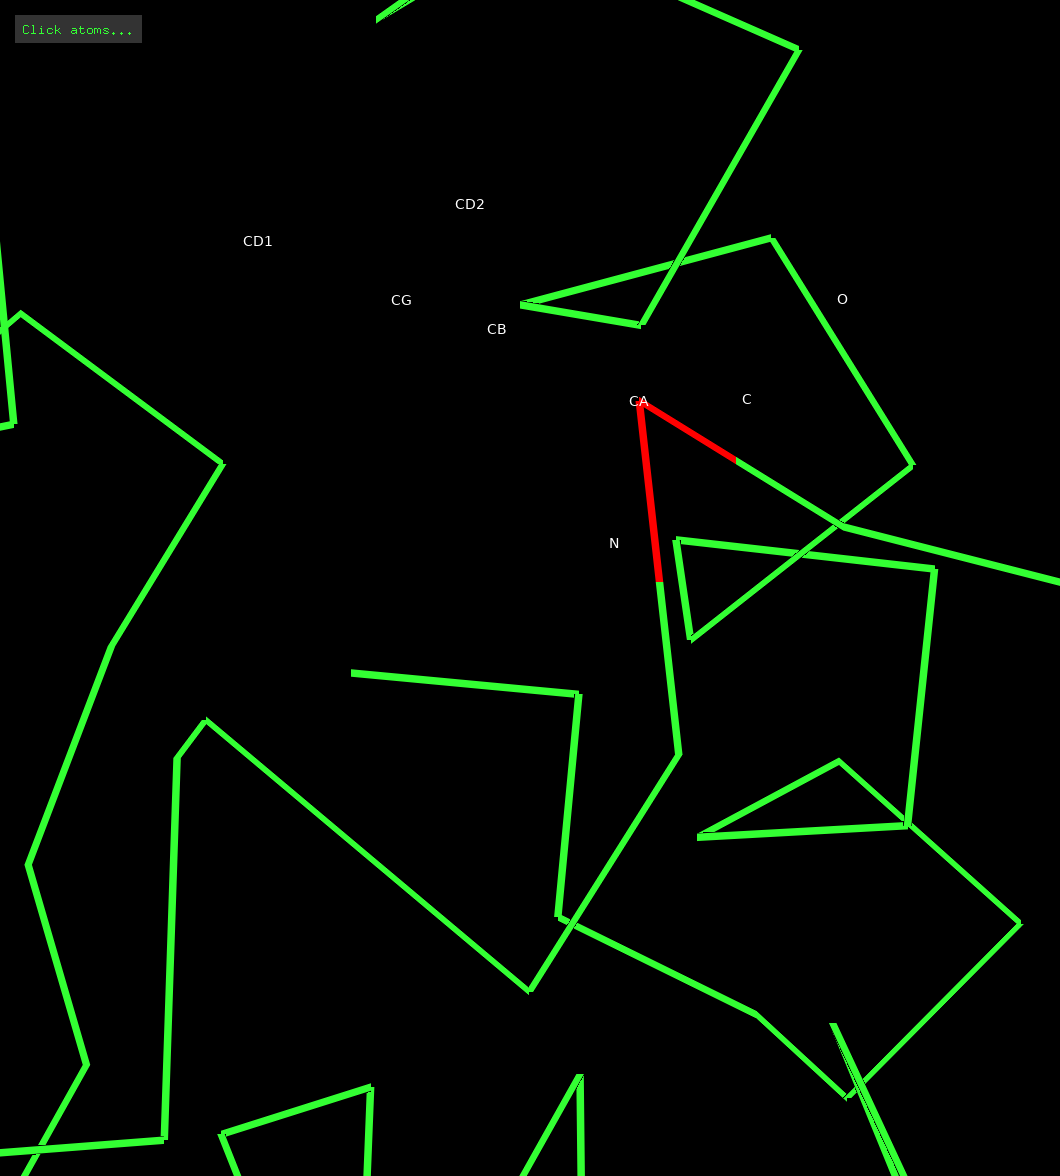
\includegraphics[width=.9\linewidth]{./ribbons.png}
\caption{Illustration of molecule with ribbons, atoms hidden but labels are in view.}
\end{figure}

\section{Problem 2}
\label{sec:org7759e29}
Since \(\beta \equiv 1/(k_{B}T)\), \(\partial \beta = -
\frac{1}{k_{B}T^{2}}\partial T\).
\begin{align}
c_{v}    & \equiv \frac{\partial <U>}{\partial T} \\
        & =  - \frac{1}{k_{B}T^{2}} \frac{\partial <U>}{\partial \beta} \\
        & =  \frac{1}{k_{B}T^{2}} \frac{\partial }{\partial \beta} (\frac{\partial ln(Z)}{\partial \beta}) \\
        & =  \frac{1}{k_{B}T^{2}} \frac{\partial }{\partial \beta} (\frac{\partial Z /\partial \beta}{Z}) \\
 & = \frac{1}{k_{B}T^{2}} \frac{\frac{\partial^{2}Z}{\partial\beta^{2}} Z - (\frac{\partial Z}{\partial\beta})^{2}}{Z^{2}} \\
 & = \frac{1}{k_{B}T^{2}} (\frac{\frac{\partial^{2}Z}{\partial\beta^{2}}}{Z} - (\frac{\partial Z}{\partial \beta} / Z)^{2}) \\
& = \frac{1}{k_{B}T^{2}} (<U^{2}> - <U>^{2})
\end{align}

For the last step, we used the fact that \(Z = \sum e^{-U\beta}\), taking
derivative with respect to \(\beta\) twice will bring down \(U^{2}\).

\section{Problem 3}
\label{sec:orgfe8ea6b}
\begin{verbatim}
begin
using Plots
epsilon_ij = 1.0
delta_ij = 4.0
V(r) = 4 * epsilon_ij * ((delta_ij/r)^12 - (delta_ij/r)^6)
r = 4:0.01:10
vs = V.(r)
plot(r,vs,title="L-J Potential",label="L-J function")
xlabel!("r\_ij Å")
ylabel!("V kJ/mol")
savefig("./potential.png")
end
\end{verbatim}

\begin{center}
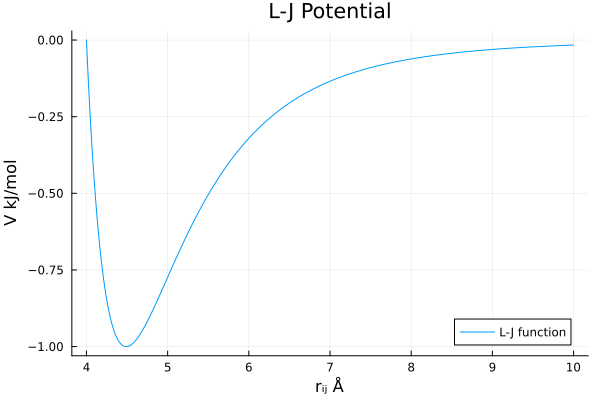
\includegraphics[width=.9\linewidth]{./potential.png}
\end{center}

\begin{verbatim}
F(r) = -98304.0 *(r^6 - 8192)/r^13
println(F(4*(2)^(1/6) + 0.5))
println(F(4*(2)^(1/6) - 0.5))
\end{verbatim}

\begin{verbatim}
F (generic function with 1 method)
-0.5989510746437929
6.2953600398067096
\end{verbatim}

\subsection{a}
\label{sec:org1de90d6}
\begin{itemize}
\item The global minimum is at \(\frac{\partial V(r_{ij})}{\partial r_{ij}} = 0\).
Solving this equation we get \(r_{ij} = 4*2^{1/6} \approx 4.4898\)
\item By definition of the force \(F = - \frac{\partial V}{\partial r}\), there
should be no force at \(r_{m}\)
\item When \(r_{ij} = r_{m} + 0.5\), \(F = - \frac{\partial V}{\partial r} =
  -0.5989510746437929\), it's attractive force, they should pull towards each
other.
\item When \(r_{ij} = r_{m} - 0.5\), \(F = - \frac{\partial V}{\partial r} =
  6.2953600398067096\), it's repulsive force, they should push them away from
each other.
\end{itemize}
\subsection{b}
\label{sec:org38c55e3}
The mixing rule says: \(\sigma_{AB} = 1/2 (\sigma_{A} + \sigma_{B}) = 4\)
angstrom. And, \(\epsilon_{AB} = \sqrt{\epsilon_{A}\epsilon_{B}} \approx 0.98
kJ/mol\)

\section{Problem 4}
\label{sec:org63c8c31}
\subsection{a}
\label{sec:org5d3adec}
\begin{itemize}
\item Bond terms: \(4 + 1 = 5\), 4 C-H and 1 C-C.
\item Angles: \(4 + 2\), 4 H-C-C, 2 H-C-H
\item Dihedrals: \(4\), 4 H-C-C-H
\end{itemize}
\subsection{b}
\label{sec:org1f34a84}
\begin{itemize}
\item For a single molecule, there are \(4\) distinct pairs of hydrogen that has 1-4
interactions.
\item For two molecules, there are \(8 + 36\) non-bonded interactions terms. \(8\)
from 1-4 interactions, and \(36\) from inter-molecular atomic interactions.
\end{itemize}

\section{Problem 5}
\label{sec:org7e3a3ac}
\begin{itemize}
\item There are three hydrogens, so the period of the potential is \(2\pi/3\).
\item The stable states occurs at \(\pi/3,\pi, 5pi/3\) angles, they are \textbf{staggered
conformation}
\item The un-stable states occurs at \(0, 2\pi/3, 4\pi/3, 2\pi\) angles, they are
\textbf{eclipsed conformation}.
\item I referenced this \href{https://www.masterorganicchemistry.com/2020/02/28/staggered-vs-eclipsed-conformations-of-ethane/}{website} to answer this question.
\item \begin{center}
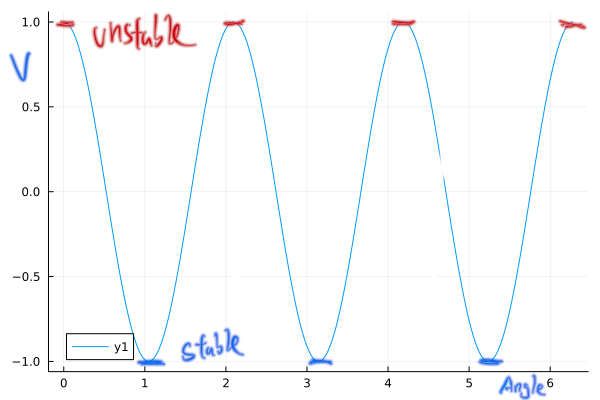
\includegraphics[width=.9\linewidth]{./periodic_potential.png}
\end{center}
\end{itemize}
\end{document}